\documentclass[../class_mech_main.tex]{subfiles}



\begin{document}

\chapter{Some Math}

% \todo{put in appendix?}

    \section{Useful Identities}
        \subsection{Differentials}
% \begin{equation}\label{eq:gradient_rvec}
%     \eqbox{
%         % \grad_{\vec{r}} \vec{r}
%         % = \grad_{\vec{r}} \sum_k r_k \unitvec{k}
%         % = \sum_k \pdv{r_k}{r_k} \unitvec{k}
%         % = \sum_k \unitvec{k}
%         % 
%         % 
%         \grad_{\vec{r}} \vec{r}
%         = \sum_k r_k \pdv_{\unitvec{k}} \vec{r}
%         = \sum_k r^k \pdv_{\unitvec{k}} \sum_l r^l \unitvec{l}
%         = \sum_{k, l} r^k \pdv{r^l}{r^k} \unitvec{l}
%         = \sum_{k, l} r^k \pdv{r^l}{r^k} \unitvec{l}
%         = \sum_{k, l} r^k \delta_k^l \unitvec{l}
%         = \vec{r}
%     }
% \end{equation}
% \todo{usually we only use gradient in classical mechanics... Not derivative of this as vector} and
% \begin{equation}
%     \eqbox{
%         \div \vec{r}
%         \hat{=} \div_{\vec{r}} \vec{r}
%         = n
%     }
% \end{equation}
% where $n$ is the number of components in $\vec{r}$ (typically $3$)


% a little more complicated:
% \begin{equation}
%     \eqbox{
%         \grad_{\vec{r}} \norm{\vec{r}}^m
%         = \grad_{\vec{r}} (\vec{r} \cdot \vec{r})^{m/2}
%         = \frac{m}{2} (\vec{r} \cdot \vec{r})^{m/2 - 1} \grad_{\vec{r}} \vec{r} \cdot \vec{r}
%         = \frac{m}{2} (\vec{r} \cdot \vec{r})^{m/2 - 1} 2 \vec{r} \cdot \grad_{\vec{r}} \vec{r}
%         \underset{Eq.~\eqref{eq:gradient_rvec}}{=} \frac{m}{2} (\vec{r} \cdot \vec{r})^{m/2 - 1} \grad_{\vec{r}} \vec{r} \cdot \vec{r}
%     }
% \end{equation}

% TODO: I do not think we actually need directional derivative of vector -> also, the subscript is not direction



\begin{align}\label{eq:gradient_rnorm}
    \eqbox{
        \grad \norm{\vec{r}}^m
    }
    &= \grad \qty(\sum_k r_k^2)^{m/2}
    \notag\\
    &= \frac{m}{2} \qty(\sum_k r_k^2)^{m/2 - 1} \grad \sum_k r_k^2
    \notag\\
    &= \frac{m}{2} \qty(\sum_k r_k^2)^{m/2 - 1} \sum_k 2 r_k \grad r_k
    \notag\\
    &= m \qty(\sum_k r_k^2)^{m/2 - 1} \sum_k r_k \sum_l \unitvec{l} \partial_l r_k
    \notag\\
    &= m \qty(\sum_k r_k^2)^{m/2 - 1} \sum_{k, l} r_k \unitvec{l} \pdv{r_k}{r_l}
    \notag\\
    &= m \qty(\sum_k r_k^2)^{m/2 - 1} \sum_{k, l} r_k \unitvec{l} \delta^k_l
    \notag\\
    &= m \qty(\sum_k r_k^2)^{m/2 - 1} \sum_k r_k \unitvec{k}
    \notag\\
    &= \eqbox{
        m \qty(\sum_k r_k^2)^{m/2 - 1} \vec{r}
    }
\end{align}




-> here is something very interesting:
\begin{equation}\label{eq:gradient_diffnorm}
    \eqbox{
        \grad_{\vec{r}} \frac{1}{\norm{\vec{r} - \vec{r}'}} = - \frac{\vec{r} - \vec{r}'}{\norm{\vec{r} - \vec{r}'}^3} = \frac{\vec{r}' - \vec{r}}{\norm{\vec{r}' - \vec{r}}^3} = - \grad_{\vec{r}'} \frac{1}{\norm{\vec{r} - \vec{r}'}}
    }
\end{equation}
where subscript denotes point of evaluation
-> this might seem puzzling since $\norm{\vec{r} - \vec{r}'} = \norm{\vec{r}' - \vec{r}}$, while $\grad_{\vec{r}} \frac{1}{\norm{\vec{r} - \vec{r}'}} = - \grad_{\vec{r}'} \frac{1}{\norm{\vec{r} - \vec{r}'}}$, but this is actually very natural; while exchanging the order of $\vec{r}, \vec{r}'$ may not change the value of the norm, it does change the associated function; basically, just ask yourself this: what happens when I change $\vec{r}$ a little bit vs.~what happens when I change $\vec{r}'$ a little bit (when evaluated in $\vec{r}$, the direction where norm gets smaller is the vector pointing from $\vec{r}$ towards $\vec{r}'$; but conversely, when evaluated in $\vec{r}'$, going in the same direction does not decrease the distance, but rather increase!); there is a sign difference in them, which translates to sign difference in the gradient, and is thus related to the direction of the respective vector in the norm
-> in essence: when evaluating in $\vec{r}$, we have to go in opposite direction of vector connecting $\vec{r}'$ and $\vec{r}$, this is why we have minus in the formula




This can be seen as a Taylor-expansion each component $\frac{a_k}{x}$, or one in $\frac{a}{x}$ if we are careful with how we write things out:
% \begin{align*}
%     \frac{1}{\norm{\unitvec{x} - \frac{a}{x} \unitvec{a}}} &\simeq \eval{\frac{1}{\norm{\unitvec{x} - \frac{a}{x} \unitvec{a}}}}_{\frac{a}{x} = 0} + \eval{\partial_{\frac{a}{x}} \frac{1}{\norm{\unitvec{x} - \frac{a}{x} \unitvec{a}}}}_{\frac{a}{x} = 0} \frac{a}{x}
%     \\
%     &= 1 + \eval{\partial_{\frac{a}{x}} \qty[(\unitvec{x} - \frac{a}{x} \unitvec{a}) \cdot (\unitvec{x} - \frac{a}{x} \unitvec{a})]^{-1/2}}_{\frac{a}{x} = 0} \frac{a}{x}
%     \\
%     &= 1 + \frac{-1}{2} \eval{\partial_{\frac{a}{x}} (\unitvec{x} - \frac{a}{x} \unitvec{a}) \cdot (\unitvec{x} - \frac{a}{x} \unitvec{a})}_{\frac{a}{x} = 0} \frac{a}{x}
%     \\
%     &= 1 + \frac{-1}{2} \eval{2 (\unitvec{x} - \frac{a}{x} \unitvec{a}) \cdot \partial_{\frac{a}{x}} (\unitvec{x} - \frac{a}{x} \unitvec{a})}_{\frac{a}{x} = 0} \frac{a}{x}
%     \\
%     &= 1 + \frac{-1}{2} \eval{2 (\unitvec{x} - \frac{a}{x} \unitvec{a}) \cdot (- \unitvec{a})}_{\frac{a}{x} = 0} \frac{a}{x}
%     \\
%     &= 1 + \unitvec{x} \cdot \unitvec{a} \frac{a}{x} = 1 + \frac{\vec{r} \cdot \vec{a}}{x^2}
% \end{align*}
% The crucial thing was to \emph{not} multiply out the $(\unitvec{x} - \frac{a}{x} \unitvec{a}) \cdot (\unitvec{x} - \frac{a}{x} \unitvec{a})$ because this would suddenly involve only $\frac{a^2}{x^2}$ and thus no vector anymore (this is fine, we can still take derivative of this, but then separately for each component $\frac{a_k}{x}$ would be required).

\todo{rather look at $\grad_{\vec{a}}$ at $\vec{a} = 0$? Then $\grad_{\vec{r}}$ follows directly, nice for field calculations below}
-> that would be wrong thing to do; what we want is Taylor-expansion with respect to $\vec{a}$ around $\vec{a} = 0$, and multi-dimensional Taylor is:
\begin{align}
    \frac{1}{\norm{\vec{r} - \vec{a}}}
    &\simeq \eval{\frac{1}{\norm{\vec{r} - \vec{a}}}}_{\vec{a} = 0}
    + \sum_k \eval{\partial_{a_k} \frac{1}{\norm{\vec{r} - \vec{a}}}}_{\vec{a} = 0} a_k
    + \frac{1}{2} \sum_{k, j} \eval{\partial_{a_j} \partial_{a_k} \frac{1}{\norm{\vec{r} - \vec{a}}}}_{\vec{a} = 0} a_k a_j
\end{align}

we can repeat most of what we did for Eq.~\eqref{eq:gradient_rnorm}:
\begin{align}
    \partial_{a_k} \frac{1}{\norm{\vec{r} - \vec{a}}}
    &= \partial_{a_k} \qty(\sum_j r_j^2 - 2 r_j a_j \cos(\theta) + a_j^2)^{-1/2}
    \notag\\
    &= \frac{-1}{2} \qty(\sum_k r_k^2 - 2 r_k a_k \cos(\theta) + a_k^2)^{-3/2} \partial_{a_k} \sum_j r_j^2 - 2 r_j a_j \cos(\theta) + a_j^2
    \notag\\
    &= \frac{-1}{2} \norm{\vec{r} - \vec{a}}^{-3} \sum_j - 2 r_j \delta_{kj} \cos(\theta) + 2 a_j \delta_{kj}
    \notag\\
    &= \norm{\vec{r} - \vec{a}}^{-3} \qty(r_k \cos(\theta) - a_k)
\end{align}
where $\theta$ is the angle between $\unitvec{r}, \unitvec{a}$.\todo{do we even need this here? We use components, no need for $\cos(\theta)$, right? Unlike for Griffiths, who expresses their scalar product as $\vec{r} \cdot \vec{a} = \norm{\vec{r}} \norm{\vec{a}} \cos(\theta)$ -> the $\cos$ would be a problem if we try to retrieve Eq.\eqref{eq:gradient_diffnorm} from it by collecting them together using basis vectors in gradient} This implies
\begin{align}
    \sum_k \eval{\partial_{a_k} \frac{1}{\norm{\vec{r} - \vec{a}}}}_{\vec{a} = 0} a_k
    &= \sum_k \norm{\vec{r}}^{-3} r_k \cos(\theta) a_k
    \notag\\
    &= \frac{\vec{r} \cdot \vec{a}}{\norm{\vec{r}}^3}
\end{align}

Based on that,
\begin{align}
    \partial_{a_m} \partial_{a_k} \frac{1}{\norm{\vec{r} - \vec{a}}}
    &= \partial_{a_m} \norm{\vec{r} - \vec{a}}^{-3} \qty(r_k \cos(\theta) - a_k)
    \notag\\
    &= \qty(r_k \cos(\theta) - a_k) \partial_{a_m} \qty(\sum_j r_j^2 - 2 r_j a_j \cos(\theta) + a_j^2)^{-3/2}
    + \norm{\vec{r} - \vec{a}}^{-3} \partial_{a_m} \qty(r_k \cos(\theta) - a_k)
    \notag\\
    &= \qty(r_k \cos(\theta) - a_k) \frac{-3}{2} \norm{\vec{r} - \vec{a}}^{-5} \partial_{a_m} \sum_j r_j^2 - 2 r_j a_j \cos(\theta) + a_j^2
    + \norm{\vec{r} - \vec{a}}^{-3} \delta_{km}
    \notag\\
    &= \qty(r_k \cos(\theta) - a_k) \frac{-3}{2} \norm{\vec{r} - \vec{a}}^{-5} \sum_j - 2 r_j \delta_{jm} \cos(\theta) + 2 a_j \delta_{jm}
    + \norm{\vec{r} - \vec{a}}^{-3} \delta_{km}
    \notag\\
    &= \qty(r_k \cos(\theta) - a_k) 3 \norm{\vec{r} - \vec{a}}^{-5} \qty(r_m \cos(\theta) - a_m)
    + \norm{\vec{r} - \vec{a}}^{-3} \delta_{km}
\end{align}
which implies
\begin{align}
    \frac{1}{2} \sum_{k, j} \eval{\partial_{a_j} \partial_{a_k} \frac{1}{\norm{\vec{r} - \vec{a}}}}_{\vec{a} = 0} a_k a_j
    &= \frac{1}{2} \sum_{k, j} r_k \cos(\theta) 3 \norm{\vec{r}}^{-5} r_j \cos(\theta) a_k a_j + \norm{\vec{r}}^{-3} \delta_{kj} a_k a_j
    \notag\\
    &= \frac{1}{2} \qty[\frac{3 (\vec{r} \cdot \vec{a}) (\vec{r} \cdot \vec{a})}{\norm{\vec{r}}^5} + \frac{\vec{a} \cdot \vec{a}}{\norm{\vec{r}}^3}]
\end{align}

Therefore we have proven that
\begin{equation}\label{eq:multipole_exp_general_calc}
    \eqbox{
        \frac{1}{\norm{\vec{r} - \vec{a}}}
        \simeq \frac{1}{x} + \frac{\vec{r} \cdot \vec{a}}{x^3} + \frac{3 (\vec{r} \cdot \vec{a})^2 - x^2 a^2}{2 x^5}
    } \, .
\end{equation}


-> apparently, this can be re-expressed in terms of Legendre polynomials; in fact, $\frac{1}{r}$ is generating function of Legendre (something like that, \cite{Griffiths_2017} treats this)





        \subsection{Functions}

\begin{equation}
    \eqbox{
        e^x = \lim_{n \rightarrow} (1 + \frac{x}{n})^n \todo{verify} = \sum_k \todo{complete expression}
    }
\end{equation}

from Euler formula $e^{i x} = \cos(x) + i \sin(x)$ this implies
\begin{align}
    &\eqbox{
        \cos(x) = \frac{1}{2} \qty(e^{i x} + e^{- i x}) = 1 - \frac{1}{2} x^2 \todo{complete expression}
    }
    \\
    &\eqbox{
        \sin(x) = \frac{1}{2 i} \qty(e^{i x} - e^{- i x}) = x - \frac{1}{3!} x^3 \todo{complete expression}
    }
\end{align}


other functions defined from combination of exponentials:
\begin{align}
    \eqbox{
        \cosh(x) = \frac{1}{2} \qty(e^{x} + e^{-x})
        \\
        \sinh(x) = \frac{1}{2} \qty(e^{x} - e^{-x})
    }
\end{align}



        \subsection{Vectors, Tensors}

\begin{equation}
    \eqbox{
        \vec{A} \cross \vec{B} = - \vec{B} \cross \vec{A}
    }
\end{equation}

\begin{equation}
    \eqbox{
        \vec{A} \cross (\vec{B} \cross \vec{C}) = (\vec{A} \cross \vec{B}) \cross \vec{C}
    }
\end{equation}

\todo{this is wrong. cross product is not associative. equation hereafter might still be true}

these two together imply
\begin{equation}
    \eqbox{
        \vec{A} \cross (\vec{B} \cross \vec{C}) = \vec{C} \cross \vec{A} \cross \vec{B}
    }
\end{equation}


\begin{equation}
    \eqbox{
        \vec{A} \cross (\vec{B} \cross \vec{C}) = \vec{b} (\vec{a} \cdot \vec{c}) - \vec{c} (\vec{a} \cdot \vec{b})
    }
\end{equation}
\enquote{bac-cab} rule


\begin{equation}
    \eqbox{
        (\vec{A} \cross \vec{B})^2 = \vec{A}^2 \vec{B}^2 - (\vec{A} \cdot \vec{B})^2
    }
\end{equation}
where squares are to be understood as scalar products


\begin{equation}
    \eqbox{
        \vec{A} = \vec{B} \cross \vec{C}
        \quad \Leftrightarrow \quad
        \vec{B} = \vec{C} \cross \vec{A}
        \quad \Leftrightarrow \quad
        \vec{C} = \vec{A} \cross \vec{B}
    }
\end{equation}
we are free to permutate in cross product (taking into account signs, depending on number of permutations done) \todo{check explicit equations} -> when in doubt, think about Cartesian
-> uahhhhhh this only works when we have vectors that are orthogonal!!!



    \section{Coordinates}

        \subsection{Curvilinear Coordinates}
basically: every coordinate system that cannot be obtained via translation or rotation from Cartesian coordinates is called \Def{curvilinear}


            \paragraph{Spherical Coordinates}
Instead of $\vec{r} = (x, y, z)$ we use $\vec{r} = (r, \theta, \phi)$. $r$ is \Def{radius}, $\theta$ is \Def{polar angle}, $\phi$ is \Def{azimuthal angle}. Here is how Cartesian coordinates can be expressed in terms of these new quantities:
\begin{equation}\label{eq:spherical_coords}
    \eqbox{
        \mqty(x \\ y \\ z) = \mqty(r \sin(\theta) \cos(\phi) \\ r \sin(\theta) \sin(\phi) \\ r \cos(\theta))
    }
\end{equation}

how to memorize this formula:

if we choose to measure polar angle $\theta$ from the $z$-axis on, then it is clear that $z \propto \cos(\theta)$ and $x, y \propto \sin(\theta)$ since things have to match for $\theta = 0$. same for azimuthal dependence $x \propto \cos(\phi), y \propto \sin(\theta)$


only $\qty{\vec{e}_r, \vec{e}_\theta, \vec{e}_\phi}$ constitutes a right-handed coordinate system (RHS), like Cartesian coordinates are as well. We can see this in Fig.~\ref{fig:spherical_cylindrical_coords} as well and this is the reason that we look at components $(r, \theta, \phi)$ instead of $(r, \phi, \theta)$





the inverse transformation can be obtained by forming appropriate combinations of $x, y, z$ from Eq.~\eqref{eq:spherical_coords}:
\begin{equation}
    \eqbox{
        \mqty(r \\ \theta \\ \phi)
        = \mqty(\sqrt{x^2 + y^2 + z^2} \\ \arctan(\frac{\sqrt{x^2 + y^2}}{z}) \\ \arctan(\frac{y}{x}))
        = \mqty(\sqrt{x^2 + y^2 + z^2} \\ \arccos(\frac{z}{\sqrt{x^2 + y^2 + z^2}}) \\ \mathrm{sgn}(y) \arccos(\frac{x}{\sqrt{x^2 + y^2 + z^2}}))
    }
\end{equation}
though one has to pay attention to quadrants and stuff, so this is actually really hard...



            \paragraph{Cylindrical Coordinates}

cylindrical are also possible, interesting alternative

\begin{equation}\label{eq:cylindrical_coords}
    \eqbox{
        \mqty(x \\ y \\ z) = \mqty(r \cos(\phi) \\ r \sin(\phi) \\ z)
    }
\end{equation}

-> these trivially reduce to polar coordinates if we only take first two components



\begin{figure}
    \centering

    \subfloat[Spherical Coordinates]{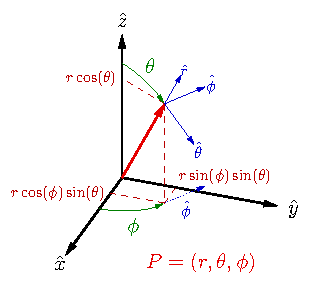
\includegraphics[width=0.42\textwidth]{pictures/spherical_coordinates.pdf}}%
    \hspace*{0.08\textwidth}%
    \subfloat[Cylindrical Coordinates]{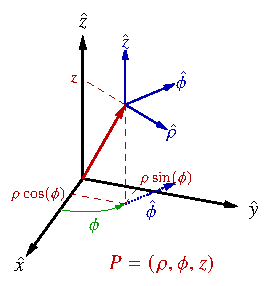
\includegraphics[width=0.38\textwidth]{pictures/cylindrical_coordinates.pdf}}

    \caption{Examples of curvilinear coordinates}
    \label{fig:spherical_cylindrical_coords}
\end{figure}



        \subsection{Differentiation Curvilinear Coordinates}
\begin{align}
	d\vec{r} &= \pdv{\vec{r}}{r} dr + \pdv{\vec{r}}{\theta} d\theta + \pdv{\vec{r}}{\phi} d\phi
	\\
	&= \unitvec{r} dr + r \unitvec{\theta} d\theta + r \sin(\theta) \unitvec{\phi} d\phi
	\\
	\Rightarrow \quad \dv{\vec{r}}{t} &= d\vec{r}(\dv{t}) = \unitvec{r} dr(\dv{t}) + r \unitvec{\theta} d\theta(\dv{t}) + r \sin(\theta) \unitvec{\phi} d\phi(\dv{t})
	\\
	&= \unitvec{r} \dv{r}{t} + r \unitvec{\theta} \dv{\theta}{t} + r \sin(\theta) \unitvec{\phi} \dv{\phi}{t}
\end{align}

\todo{just state results here, text is already nicer in next subsection}


more systematically (makes it easier to get things like second derivative):
\begin{align}
    d\vec{r}
    &= d\mqty(r \sin(\theta) \cos(\phi) \\ r \sin(\theta) \sin(\phi) \\ r \cos(\theta))
    \notag\\
    &= \mqty(d[r \sin(\theta) \cos(\phi)] \\ d[r \sin(\theta) \sin(\phi)] \\ d[r \cos(\theta)])
    \notag\\
    &= \mqty(dr \sin(\theta) \cos(\phi) + r d\sin(\theta) \cos(\phi) + r \sin(\theta) d\cos(\phi) \\ dr \sin(\theta) \sin(\phi) + r d\sin(\theta) \sin(\phi) + r \sin(\theta) d\sin(\phi) \\ dr \cos(\theta) + r d\cos(\theta))
    \notag\\
    &= \mqty(dr \sin(\theta) \cos(\phi) + r \cos(\theta) d\theta \cos(\phi) + r \sin(\theta) (-\sin(\phi)) d\phi \\ dr \sin(\theta) \sin(\phi) + r \cos(\theta) d\theta \sin(\phi) + r \sin(\theta) \cos(\phi) d\phi \\ dr \cos(\theta) + r (-\sin(\theta)) d\theta)
    \notag\\
    &= \mqty(\sin(\theta) \cos(\phi) \\ \sin(\theta) \sin(\phi) \\ \cos(\theta)) dr
    + \mqty(r \cos(\theta) \cos(\phi) \\ r \cos(\theta) \sin(\phi) \\ - r \sin(\theta)) d\theta
    + \mqty(- r \sin(\theta) \sin(\phi) \\ r \sin(\theta) \cos(\phi) \\ 0) d\phi
    \notag
\end{align}
% Eq.~(71) from \url{https://mathworld.wolfram.com/SphericalCoordinates.html} -> but he has switched $\theta, \phi$

We know that this must read $d\vec{r} = a \unitvec{r} dr + b \unitvec{\theta} d\theta + c \unitvec{\phi} d\phi$ for some factors $a, b, c$ (since $d\vec{r}(\unitvec{\theta}) = d\vec{r}(\dv{\theta}) = \dv{\vec{r}}{\theta}$ and $\dv{r}{\theta} = 0 = \dv{\phi}{\theta}$)
\begin{enumerate}[1.]
    \item The coefficient of $dr$ is already unit, meaning
    \begin{equation}
        \eqbox{
            \unitvec{r} = \mqty(\sin(\theta) \cos(\phi) \\ \sin(\theta) \sin(\phi) \\ \cos(\theta))
        }
    \end{equation}


    \item The coefficient of $d\theta$ has norm $r$, so that
    \begin{equation}
        \eqbox{
            \unitvec{\theta} = \mqty(r \cos(\theta) \cos(\phi) \\ r \cos(\theta) \sin(\phi) \\ - r \sin(\theta)) 
        }
    \end{equation}
    and the coefficient itself is $r \unitvec{\theta}$


    \item The coefficient of $d\phi$ has norm $r \sin(\theta)$, so that
    \begin{equation}
        \eqbox{
            \unitvec{\phi} = \mqty(- r \sin(\theta) \sin(\phi) \\ r \sin(\theta) \cos(\phi) \\ 0)
        }
    \end{equation}
    and the coefficient itself is $r \sin(\theta) \unitvec{\phi}$
\end{enumerate}
(Basic idea to find norm: look out for terms that are common in all components, these do not cancel. All others actually cancel because of $\sin[2](x) + \cos[2](x) = 1$ and it is only these type of terms that are left after we remove common terms.) Therefore,
\begin{equation}\label{eq:spherical_coords_deriv}
    \eqbox{
        d\vec{r} = \unitvec{r} + r \unitvec{\theta} + r \sin(\theta) \unitvec{\phi}
    }
\end{equation}
A general formula for the unit vectors is
\begin{equation}
    \eqbox{
        \unitvec{k} = \flatfrac{\dv{\vec{r}}{k}}{\norm{\dv{\vec{r}}{k}}}
    }
\end{equation}


Sanity check that these formulas are correct: verify from Fig.~\ref{fig:spherical_cylindrical_coords} (a) that upon a step of, e.g., $d\theta$, the actual step made in Cartesian coordinates is $r d\theta$ (perhaps, Fig.~\ref{fig:spherical_coords_are_vol_el} are helpful here as well)


These coefficients also yield, very naturally, how the gradient must look like in spherical coordinates:
\begin{equation}
    \eqbox{
        \grad = \unitvec{r} \pdv{r} + \frac{1}{r} \unitvec{\theta} \pdv{\theta} + \frac{1}{r \sin(\theta)} \unitvec{\phi} \pdv{\phi}
    } \, .
\end{equation}
Basically, this expression has correction factors implemented for what we know is going to \enquote{come out} the derivatives of the curvilinear components.



        \subsection{Areas \& Volumes in Curvilinear Coordinates}

volume element is $dV = dx \, dy \, dz$, with transformation into curvilinear coordinates applied; but we do not want to calculate this explicitly, too nasty, so we look at plot instead (Fig.~\ref{fig:spherical_coords_are_vol_el} (b)). volume element has thickness $dr$ in radial direction; in polar direction we cut out a piece of length $d\theta$ from a circle with circumference $r$; in azimuthal direction, we cut out a piece of length $d\phi$ from a circle of radius $r \sin(\theta)$ (different radius compared to polar direction is easily explained, for polar we rotate the whole vector basically, but for azimuthal we must keep the $z$-component fixed; and just like we can find radius of polar circle by noticing that it goes through $z$-axis $\equiv (0, 0, r)$, we find radius of azimuthal circle by noticing it goes through $x$-axis $\equiv (r \sin(\theta), 0, 0)$, or equivalently through $y$-axis $\equiv (0, r \sin(\theta), 0)$); forming the product of these three yields the correct result,
\begin{equation}
    \eqbox{
        dV = \norm{d\vec{r}} = dr \, r d\theta \, r \sin(\theta) d\phi = r^2 \sin(\theta) \, dr \, d\theta \, d\phi
    }
\end{equation}


-> better justification for this: now, say we start at some position $\vec{r}$ and then go a step $dx$, then $dy$, then $dz$; this will form shape that can be completed to a cube basically and volume of this (infinitesimal) cube is $dV = dx \, dy \, dz$; but if we go $dr$, then $d\theta$, then $d\phi$, what we end up with is a shape that does \emph{not} have volume $dV = dr \, d\theta \, d\phi$; from plot, this makes sense, because length that we move when making step $d\phi$ for example from some position $\vec{r}$ actually depends on the position now; this is an effect of being in curvilinear coordinates and we have to use correction factor to account for this in $dV$ (this factor is called Jacobi determinant); more explicitly, this is idea: $(r, \theta, \phi + d\phi) - (r, \theta, \phi) \neq (0, 0, d\phi)$ \todo{verify this is actually true and related to Jacobi; should be, though -> ah, maybe idea is $x(r, \theta, \phi + d\phi) - x(r, \theta, \phi)$ is dependent on point and does not reduce to constant multiplied by $d\phi$ (?)}, an infinitesimal step works different in these types of coordinates; basically, when I make step $d\phi$ from $\vec{r}$, then the actual step I make (= length of step in Cartesian) is $r \sin(\theta) d\phi$
% $(r + dr, \theta + d\theta, \phi + d\phi) - (r, \theta, \phi) \neq (dr, d\theta, d\phi)$ -> overkill here, since all couple with each other, right?
-> just say: we plot $(r, \theta, \phi)$ and $(r, \theta, \phi + d\phi$); expectation: angular step we have to make to connect them is simply $d\phi$; but this is not true, actually we have to make $r \sin(\theta) d\phi$ -> maybe "angular step" is wrong word here (I refer to arclength of circle that connects them; this is path following $\vec{e}_\phi$ between the two points, i.e.~how we would compute the distance in components basically), but idea is certainly true! And perhaps simplest way to explain, do not try to use differences of components here -> though $(r, \theta, \phi + d\phi) - (r, \theta, \phi) \neq (0, 0, d\phi)$ might actually be true, now that I see argument with $\vec{e}_\phi$ here, this is exactly what we say there, don't we?
-> key idea is really: in Cartesian, when drawing $(x,y,z)$ and $(x+dx,y+dy,z+dz)$, then their distance in each direction really is the corresponding infinitesimal step; but when I draw $(r, \theta, \phi)$ and $(r, \theta, \phi + d\phi)$, then the step I have to make is not than $d\phi$, but depends on point (obvious from plot, but non-trivial when we try to write this down as expression involving components; SO REALLY DO NOT TRY)



-> crucial part: when we take as axes the three vectors $\vec{e}_r, \vec{e}_\theta, \vec{e}_\phi$, then the separation of $(r, \theta, \phi)$ and $(r, \theta, \phi + d\phi)$ is actually $d\theta$ (actually norm of their difference as well); however, what we are usually interested in for our physical analysis is the distance between points in Euclidean space; now, for Cartesian coordinates, this is trivially computed as $d(x_1, x_2) = \norm{x_1 - x_2} = \sqrt{\sum_i (x_{1, i} - x_{2, i})^2}$, but that does not mean this is true in spherical coordinates! To see why, let us plot $(r, \theta, \phi)$ along with differential steps in all directions and check which volume element this cuts out


$g = J^T J = \mqty(\dmat{1 \\ r \\ r \sin(\theta)})$



from this we get area element easily, just don't multiply with $dr$ (which can be seen as differentiation with respect to $dr$):
\begin{equation}
    \eqbox{
        dA = r d\theta \, r \sin(\theta) d\phi = r^2 \sin(\theta) \, d\theta \, d\phi
    }
\end{equation}



\begin{figure}
    \centering

    \subfloat[Area Element]{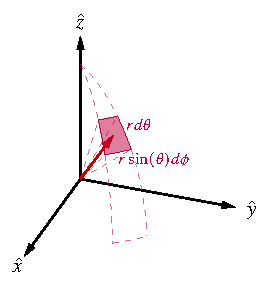
\includegraphics[width=0.42\textwidth]{pictures/spherical_coordinates_area_el.pdf}}%
    \hspace*{0.08\textwidth}%
    \subfloat[Volume Element]{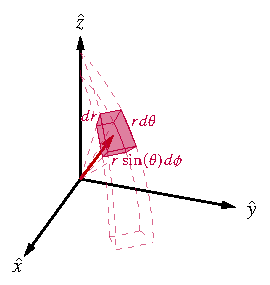
\includegraphics[width=0.38\textwidth]{pictures/spherical_coordinates_vol_el.pdf}}

    \caption{Area and volume element in spherical coordinates.}
    \label{fig:spherical_coords_are_vol_el}
\end{figure}



        \subsection{Polar Coordinates}


polar coordinates are just spherical coordinates (Eq.~\eqref{eq:spherical_coords}) with $\theta = 90\degree$ (and we get $dA$ from $dV$ by formally setting $d\theta = 1$) -> thus trick: remember spherical coordinates, then how they reduce

-> alternatively, cylindrical with $z = 1$


\begin{equation}\label{eq:polar_coords}
    \eqbox{
        \mqty(x \\ y) = \mqty(r \cos(\phi) \\ r \sin(\phi))
    }
\end{equation}



\begin{figure}
    \centering

    \subfloat[Definition]{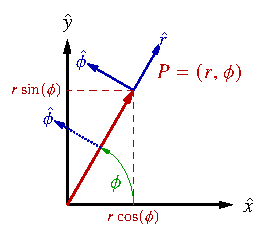
\includegraphics[width=0.42\textwidth]{pictures/polar_coordinates.pdf}}%
    \hspace*{0.08\textwidth}%
    \subfloat[Area Element]{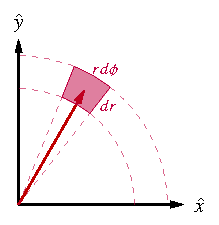
\includegraphics[width=0.38\textwidth]{pictures/polar_coordinates_area_el.pdf}}

    \caption{Polar Coordinates}
    \label{fig:polar_coordinates}
\end{figure}



    \section{Differential Equations}
-> note: just as something general to remember, order of differential equations is the number of constants that appear during integration of equation to obtain solution; this is sanity check for solution!



    \section{Differential Geometry}
    \label{sec:diff_geo}
we take approach inspired by Thorne+Blandford: cite relatively advanced math, trading elegance and robustness of expressions for readibility if one is not familiar with some advanced calculus (mainly)


in 1.8 of Thorne+Blandford, they explain connection between differential conservation laws and corresponding integration laws


definition of gradient of a function: components of differential, i.e.
\begin{equation}
    \eqbox{
        df = \langle \grad f, d\vec{x} \rangle = \sum_i \pdv{f}{x^i} dx_i
    }
\end{equation}

-> this can be generalized to tensors of arbitrary rank by means of covariant derivative (cf.~Thorne+Blandford)



note: partial derivative with respect to time $t$ is \emph{not} same as total (true for any other variable as well)! For example, if $F = k x(t)$, then $\pdv{F}{t} = 0$ because time does not explicitly appear in there; but $dF = \pdv{F}{x} dx$, so $\dv{F}{t} = \pdv{F}{x} \dv{x}{t}$ \todo{right?}



Stokes' theorem is all you need to know in order to remember how to connect differential conservation laws and corresponding integration laws (Gauß, Stokes, Green, fundamental theorem of calculus) -> cf.~1.8 of Thorne+Blandford

\begin{thm}[(Generalized) Stokes' Theorem]
    For orientable manifold $M$ with boundary $\partial M$
    \begin{equation}
        \eqbox{
            \int_M d\omega = \int_{\partial M} \omega
        }
    \end{equation}
\end{thm}




Hodge duality formalizes identification of are element $dA$ with normal vector of this are, e.g., $* dx = dy \wedge dz \equiv dA$ -> explains components of rotation, right? See H\_Analysis, page 203 (Beispiel 6.22)

-> for 1-form $g = g_\mu dx^\mu = \langle \vec{g}, d\vec{x} \rangle$, we have $dg = d \langle \vec{g}, d\vec{x} \rangle = \langle \curl \vec{g}, * d\vec{x} \rangle$. So demanding $g$ is conservative amounts to demanding the good-old condition of vanishing curl


rule to memorize laws: we need $n$-differential form to be able to integrate on $n$-dimensional manifold. So we need something with a single coefficient for this ($n$-form only has one; $n - 1$-form would have two coefficients etc), and curl as vectorial quantity would have three, so we need divergence as scalar quantity serving as single coefficient here


nice to memorize area integral: $\int_S \vec{v} \, d\vec{A} = \int v_x \, \hodge dx + \int v_y \, \hodge dy + \int v_z \hodge dz$ -> integrate components over area to which unit vector for this component is the normal vector (we get this area from normal vector using hodge star) \todo{check how components of normal vector enter here, there should be some kind of inner product with it involved...} -> we want flux of vector field through the surface, so we must extract component that flows through the surface, which is done via projection onto normal vector ($d\vec{S}$ is just notation); after that it is just surface integral of scalar function with area element $dS$


H\_Analysis, Beispiel 6.47

\begin{ex}[Gauß's Law/Theorem]
    $M = \mathbb{R}^3$ or rather subset thereof

    note that $dV$ and $d^3x$ are the same
\end{ex}


\begin{ex}[Stokes' Theorem]
    $M = \mathbb{R}^2$ or rather subset thereof
\end{ex}


\begin{ex}[Fundamental Theorem of Calculus]
    $M = \mathbb{R}$ or subset thereof
\end{ex}


\begin{ex}[Green's Law/Theorem]
    hmmm what is $M$ here?
\end{ex}


-> using $\oint$ instead of $\int$ indicates that we assume closed curve/surface




another important law is Gauß's law (\emph{another} Gauß law...):
\begin{equation}
    \eqbox{
        \delta(\vec{r} - \vec{r}_0) = \frac{-1}{4 \pi} \nabla^2 \frac{1}{\norm{\vec{r} - \vec{r}_0}}
    }
\end{equation}



\begin{thm}[Helmholtz Theorem]\label{thm:helmholtz_thm}
    If the divergence $\div \vec{F} \eqqcolon D(\vec{r})$ and the curl $\curl \vec{F} \eqqcolon \vec{C}(\vec{r})$ of a vector function $\vec{F}(\vec{r})$ are specified, and if they both go to zero faster than $1/r^2$ as $r \rightarrow \infty$, and if $\vec{F}(\vec{r})$ goes to zero as $r \rightarrow \infty$, then $\vec{F}$ is given uniquely by
    \begin{equation}
        \eqbox{
            \vec{F} = - \grad U + \curl \vec{W}
        }
    \end{equation}
    where
    \begin{equation}
        \eqbox{
            U(\vec{r}) = \frac{1}{4\pi} \int \frac{D(\vec{r}')}{\norm{\vec{r} - \vec{r}'}} \, dV'
        }
        \eqbox{
            \vec{W}(\vec{r}) = \frac{1}{4\pi} \int \frac{\vec{C}(\vec{r}')}{\norm{\vec{r} - \vec{r}'}} \, dV'
        }
    \end{equation}
    are integrals over the entire space.
\end{thm}




    \section{Calculus Of Variations}

displacements are considered instantaneous, meaning
\begin{equation}
    \eqbox{
        \delta t = 0
    }
\end{equation}
Moreover (Thornton+Marion, Eq.(7.132)),
\begin{equation}
    \eqbox{
        \delta \dot{x}_i = \delta \dv{x_i}{t} = \dv{t} \delta x_i = 0
    }
\end{equation}


any variation $\delta$ is usually expressed in terms of a derivative $\pdv{\alpha}$; therefore, it is not surprising that we have something like a chain rule for it:
\begin{equation}
    \eqbox{
        \delta H(q_i, p_i) = \sum_i \pdv{L}{q_i} \delta q_i + \pdv{H}{p_i} \delta p_i
    }
\end{equation}



difference to derivative: variation is applied to a function of functions (a functional), i.e.~the result is not a point (the way it is for derivative), but rather a whole function

-> i.e.~for $J = J[f(x), g(x)]$,
\begin{equation}
    \eqbox{
        \delta J \coloneqq \eval{\dv{\epsilon} J'[f(x), g(x)]}_{\epsilon = 0} = \eval{\dv{\epsilon} J[f(x) + \epsilon h(x), g(x) + \epsilon h'(x)]}_{\epsilon = 0}
    }
\end{equation}

-> I guess in modern mathematics, we can argue that a function is also just a point in a space (?)


\end{document}